% IEEE Conference Paper - SIF Paper Draft
\documentclass[conference]{./template/IEEEtran}

\usepackage[T1]{fontenc}
\usepackage{cite}
\usepackage{amsmath,amssymb,amsfonts}
\usepackage{algorithmic}
\usepackage{graphicx}
\usepackage{textcomp}
\usepackage{xcolor}
\usepackage{tikz}
\usepackage{forest}
\usetikzlibrary{arrows.meta,positioning,shapes,calc,decorations.pathreplacing}
\usepackage{listings}
\usepackage{array}
\usepackage{booktabs}
\newcolumntype{C}[1]{>{\centering\arraybackslash}p{#1}}
\newcommand{\lightrule}{\noindent\textcolor{black!30}{\rule{0.97\columnwidth}{0.4pt}}}
\newlength{\vizsep}\setlength{\vizsep}{0.35cm}
\newlength{\vizseplg}\setlength{\vizseplg}{0.5cm}
\lstset{
  basicstyle=\ttfamily\small,
  keywordstyle=\bfseries,
  language=Python,
  frame=single,
  breaklines=true
}

\begin{document}

\title{Symbolic Execution is (Not Quite) All You Need}

\author{
\IEEEauthorblockN{Sophie Smithburg}
\thanks{This paper and its Lean 4 mechanization were developed with extensive use of Claude Code and ChatGPT, some use of Codex CLI, and a smattering of other LLM tools in earlier prototypes.}
}

\maketitle

\begin{abstract}
Given a programming language implementation running on a host machine and a grammar, you can use symbolic execution and formal ISA semantics as oracles to extract a formal labeled transition system that simulates the implementation's behavior.

In plain terms: You can automatically derive executable formal specs from implementations---no one writes specs, everyone writes implementations, but you can't prove things about implementations directly. This technique lets you get the spec from the implementation (given its grammar).
\end{abstract}

\begin{IEEEkeywords}
symbolic execution, formal verification, labeled transition systems, semantic extraction, grammar mining, Lean 4
\end{IEEEkeywords}

%%%%%%%%%%%%%%%%%%%%%%%%%%%%%%%%%%%%%%%%%%%%%%%%%%%%%%%%%%%%%%%%%%%%%%%%%%%%%%%
\section{Introduction}
%%%%%%%%%%%%%%%%%%%%%%%%%%%%%%%%%%%%%%%%%%%%%%%%%%%%%%%%%%%%%%%%%%%%%%%%%%%%%%%

% SOURCE: intro-sources-and-draft.md:76-78 (Synthetic Draft - Sophie's words)
% Provenance: 100% Sophie's words from Bluesky threads
% Minor edits: "it's" -> "its", added "We", "in the form" (was "in form")

We can model a programming language executing on a host machine as a host labeled transition system $H$~\cite{henzinger2000symbolic} which, after having been fed $\mathcal{I}$, the implementation, simulates $G$---this is to say the PL is $G$, its implementation is $\mathcal{I}$, and the host machine is $H$. If we observe a set of traces $\tau \in \mathcal{T}$ of executions of $G$ recorded at the level of $H$, we can use a specific algorithm to extract an LTS $G'$ that simulates $H_\mathcal{I}$.

In concrete terms, one can think of $H$ as something like x86 or ARM, and $\mathcal{I}$ as something like CPython or V8. This matters because in practice everyone builds implementations. No one writes specs, but you can't prove things about implementations directly for the most part, and you can about specs. So in order to have an effective ratchet in the sense of the LangSec 2017 Perry Metzger talk, we want to be able to get these specs for these implementations.

To prove $G'$ faithfully captures $G$, we would need $G$ in a formalism that shares the same proof basis as $G'$---but in practice, this is never the case. The problem we're trying to solve practically speaking is inferring $G'$ when no one cares to actually write out $G$, they're all focused on $\mathcal{I}$. So what we do instead is prove that $G'$ simulates $H_\mathcal{I}$, the LTS $H$ after executing $\mathcal{I}$, by way of quotienting over all the implementation details of $H$ that aren't causally controllable by way of inputs to $G$ in the form of program structure or codata.

%%%%%%%%%%%%%%%%%%%%%%%%%%%%%%%%%%%%%%%%%%%%%%%%%%%%%%%%%%%%%%%%%%%%%%%%%%%%%%%
\section{Notation}
%%%%%%%%%%%%%%%%%%%%%%%%%%%%%%%%%%%%%%%%%%%%%%%%%%%%%%%%%%%%%%%%%%%%%%%%%%%%%%%

\begin{itemize}
% === EXISTING NOTATION (from main.tex - Sophie wrote these) ===
\item $\Sigma$ is the concrete runtime space, and in our case, it is parametric over the definition of an ISA\@. It's basically the main memory, registers, CPU flags, any state that is documented for a particular CPU or host machine. In the more abstract view of a labeled transition system, which we focus on in this paper, $\Sigma$ is simply the state space of $H$.
\item $X$ is computed indirectly, but can be defined directly. $X$ is the set of all the state of the subsystem (like the programming language under analysis) that can be controlled by a program in that programming language. In the mechanization, configurations are concretely the function type $\text{Dim} \to \text{Value}$: dimension-indexed observations of host state. The configuration space $X$ is the image of $\pi$ within this type. It is possible to extend this in the future to include input by way of any predefined input channel, but modeling codata introduces non-determinism, which is out of scope for the current paper.
\item $\pi$ is the mapping from $\Sigma$ to $X$, which we get precisely by the indirect computation mechanism hinted at above.
\item $H$ is the host machine, it can be seen as an LTS or a bog standard ISA
\item $G$ is the true transition system, or notionally, what would be the specification of the programming language if the programming language were defined by the implementation? In some very real sense, a lot of programming languages are. Take, for example, C, Python, and the fact that it's been stated about the specifications in the Python enhancement proposal process and other documents in the standard that if one were to follow them, it's likely, without other guidance, they would end up with an entirely different language.
\item $\mathcal{I}$ is the programming language implementation under analysis
% H_I: Sophie's phrase "the LTS H after executing I" + Claude added "the host machine primed with the implementation"
\item $H_\mathcal{I}$ is the LTS $H$ after executing $\mathcal{I}$---i.e., an x86 machine after executing the CPython binary, or an ARM machine after executing a V8 implementation
\item $G'$ is the transition system we extract from traces $\tau \in \mathcal{T}$ of running $H_\mathcal{I}$, i.e.\ the host machine $H$ or host labeled transition system without loss of generality. Additionally, $G'$ is composed from $R$.
\item $\Gamma$ is the formal grammar for $\mathcal{I}$. We require only that $\Gamma$ has finitely many nonterminals and that $H_\mathcal{I}$'s transitions are labeled by $\Gamma$'s rules (grammar conformance).
\item $\gamma \in \Gamma$ is a production in the grammar
\item $\text{holes}(\gamma)$ is the set of holes in production $\gamma$
\item $\kappa_h$ is the sentinel value for hole $h$ in production $\gamma$
\item $\mathcal{C}$ is a covering set of programs that enumerate all productions in $\Gamma$, and alternatives in each production, in a minimized way to be elaborated upon later
\item $\tau \in \mathcal{T}$ is a trace, or a sequence of states and labels for the transitions between them, generated when we run the host machine $H$ over the programming language implementation $\mathcal{I}$ and a program from $\mathcal{C}$, which implies all the values relevant to updates (it is of course more convenient when the values for updates are provided for us; we presume this, we think without loss of generality, but perhaps that's wrong!)
\item $\mathcal{T}$ is the set of all traces $\tau$
\item The semantics of any production decomposes into a sequence of deterministic steps between its holes. A \textbf{Hole-to-Hole (HTH) block} is one such step: given $h_i, h_j \in \text{holes}(\gamma)$ consecutive in evaluation order, the HTH block $\ell = (\gamma, h_i, \gamma, h_j)$ is the unique non-branching execution segment from $h_i$'s evaluation to $h_j$'s (Figure~\ref{fig:hth-block}). These are the units over which we extract relational transformers $R_\ell$; their lack of internal branching makes symbolic execution tractable.
\item $L$ is the set of HTH labels; each $\ell = (\gamma_s, h_i, \gamma_d, h_j)$ identifies the transition from hole $h_i$ in production $\gamma_s$ to hole $h_j$ in production $\gamma_d$, where $h_i \in \text{holes}(\gamma_s)$ and $h_j \in \text{holes}(\gamma_d)$ are consecutive in evaluation order. In the common intra-production case, $\gamma_s = \gamma_d$; cross-production transitions have $\gamma_s \neq \gamma_d$
\item $\ell \in L$ is a label for a step in our transition system, identifying which HTH region the step corresponds to
\item $R_\ell(x, x') := \text{Guard}_\ell(x) \land \text{Update}_\ell(x, x')$ summarizes the preconditions and state transformations for a step labeled $\ell$
\item $R = \{R_\ell\}_{\ell \in L}$ is the family of relational summaries over all HTH labels

% === OBSERVATION + CONTROLLABILITY (from Lean mechanization) ===
\item $\text{observe} : \Sigma \to \text{Dim} \to \text{Value}$ is the observation function mapping host states to per-dimension observable values. The projection $\pi$ is defined in terms of $\text{observe}$ by restricting to tracked dimensions $X$
\item \textbf{Observation faithfulness} ($h_\text{faithful}$): $\forall \sigma_1, \sigma_2.\; \sigma_1 \in \text{Reach}(H_\mathcal{I}) \implies (\forall d.\; \text{observe}(\sigma_1, d) = \text{observe}(\sigma_2, d)) \implies \sigma_1 = \sigma_2$. The observation function is injective on reachable states: any reachable host state is uniquely determined by its observations among all states, not just other reachable ones---$\sigma_2$ is unconstrained. This asymmetry is necessary because $\text{IsXControllable}$ quantifies over all states in the fiber $\pi^{-1}(\pi(\sigma))$, including unreachable ones. Two unreachable states need not be distinguished from each other. This is the key hypothesis enabling co-refinement convergence (Section~V).
\item \textbf{X-controllability.} A label $\ell$ is \emph{X-controllable} at state $\sigma$ if $\ell$ is enabled throughout the fiber $\pi^{-1}(\pi(\sigma))$---that is, every host state with the same projected configuration can take the transition. This formalizes the concept underlying $\text{Alt}(s)$: X-controllable transitions are those whose firing depends only on $X$-visible state.

% === ORACLE NOTATION ===
% SOURCE: Sophie dictation 2026-01-10 (VERBATIM)
\item $\text{Reach}(H_\mathcal{I})$ is the set of reachable states in $H_\mathcal{I}$
\item $\text{BStates}(\mathcal{I}) \subseteq \text{Reach}(H_\mathcal{I})$ is the set of \emph{all} reachable states with branching behavior---i.e., $s \in \text{BStates}(\mathcal{I})$ iff $|\text{Alt}(s)| > 1$. The branching oracle $O$ discovers these via symbolic execution combined with formal ISA semantics (e.g., K framework reachability logic), both operating at the $\Sigma$ level.
% DRAFT: Alt(s) refined - all feasible outcomes reachable by modifying π(s)
\item $\text{Alt}(s)$ is the set of \emph{all} feasible branch outcomes from state $s$ that are reachable by modifying $\pi(s)$. This is the completeness constraint: if outcome $o$ is achievable by changing $X$-state at $s$, then $o \in \text{Alt}(s)$. Branches depending on state outside $X$ are either implementation-internal (irrelevant to $G'$) or trigger $\pi$-refinement to include that state.
% DRAFT: O(s) produces constraints over π to achieve alternatives
\item $O(s)$ is the branching oracle: given $s \in \text{BStates}(\mathcal{I})$, it produces constraints at the $\Sigma$ level that achieve each alternative in $\text{Alt}(s)$, which are then lifted to constraints over $\pi(s)$
% DRAFT: ReplayApply applies constraint to π, runs to get branch outcome
\item $\text{ReplayApply}(s, c) \Downarrow o$ means replaying from state $s$ with $\pi(s)$ modified by constraint $c$ realizes branch outcome $o$
% DRAFT: O* is fixpoint of both traces AND π refinement - up to behavioral equivalence
\item $O^*(\mathcal{T})$ is the fixpoint up to behavioral equivalence: for each branch outcome $o \in \text{Alt}(s)$ at each $s$ along traces in $O^*(\mathcal{T})$, we require \emph{at least one exemplar trace} realizing $o$. We do not generate all traces---only one representative per behavioral pattern (same control flow, same HTH structure). Additionally, $\pi$ has stabilized. This suffices for completeness: every reachable behavior has an exemplar from which we extract $R_\ell$.

% === SIMULATION ===
% SOURCE: Sophie dictation 2026-01-10 (VERBATIM)
\item $G' \preceq M$ states that $G'$ simulates $M$, which is to say that all behaviors of $M$ have corresponding behaviors in $G'$~\cite{vanglabbeek1990ltbt,vanglabbeek1993ltbt2}
\end{itemize}

\begin{figure}[t]
\centering
\resizebox{0.95\columnwidth}{!}{%
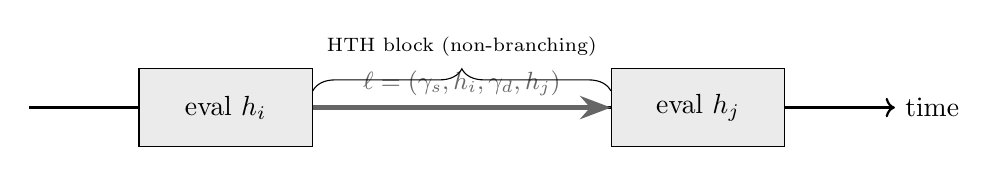
\begin{tikzpicture}
\draw[thick,->] (-0.5,0) -- (10.5,0) node[right] {time};
\node[draw,fill=black!8,minimum height=10mm,minimum width=22mm] (e1) at (2,0) {eval $h_i$};
\node[draw,fill=black!8,minimum height=10mm,minimum width=22mm] (e2) at (8,0) {eval $h_j$};
\draw[-{Stealth},black!60,line width=1.8pt] (e1.east) -- (e2.west)
  node[midway,above,font=\small] {$\ell = (\gamma_s,h_i,\gamma_d,h_j)$};
\draw[decorate,decoration={brace,amplitude=8pt,raise=6pt}]
  (e1.east) -- (e2.west)
  node[midway,above=15pt,font=\scriptsize] {HTH block (non-branching)};
\end{tikzpicture}%
}
\caption{Hole-to-Hole (HTH) block as the execution segment between consecutive hole evaluations.}
\label{fig:hth-block}
\end{figure}

%%%%%%%%%%%%%%%%%%%%%%%%%%%%%%%%%%%%%%%%%%%%%%%%%%%%%%%%%%%%%%%%%%%%%%%%%%%%%%%
\section{Main Claim}
%%%%%%%%%%%%%%%%%%%%%%%%%%%%%%%%%%%%%%%%%%%%%%%%%%%%%%%%%%%%%%%%%%%%%%%%%%%%%%%

% SOURCE: intro-sources-and-draft.md:82 (Sophie's words)
% Provenance: 100% Sophie's words from Bluesky

We reconstruct behavior piecewise along traces and each trace is a sound reconstruction because it almost literally replays the trace we saw. And also we use a model of the host machine that knows about branches to achieve completeness by adding new traces for all uncovered paths. If you manage soundness and completeness of reconstruction that's basically the whole game.

\subsection{Oracles}

We require two kinds of oracles: one for branching behavior and one for value transformations. Neither is counterfactual---both are instantiated by real tools.

\subsubsection{Branching}

The branching oracles we require are in no way counterfactual. Some aspects are partially captured by symbolic execution and then the rest of that is fully captured by formal ISA semantics.
Throughout this paper, the ``branching oracle $O$'' refers to this combined realization---selective symbolic execution for path feasibility plus formal ISA semantics (e.g., the K framework~\cite{rosu2010kframework}) for reachability---not an additional assumption beyond symex. We use $O$ as notational shorthand.

\paragraph{Completeness.}
% SOURCE: ChatGPT axiom screenshot, formalizing Sophie's "completeness by covering all branches"
For all $\mathcal{I}$-relevant branch states and all feasible outcomes, the oracle can produce a constraint that achieves that outcome:
\[
\forall s \in \text{BStates}(\mathcal{I}).\; \forall o \in \text{Alt}(s).\; \exists c \in O(s).\; \text{ReplayApply}(s, c) \Downarrow o
\]

\subsubsection{Value Transformation}

What we need for value transformation inference is provided fully by symbolic execution engines. When symbolically executing a basic block, the engine produces symbolic expressions showing how input values map to output values---this directly gives us the $\text{Update}(x, x')$ component of each $R_\ell$~\cite{voogd2025compositional,loow2025compositional}.

\subsection{Proof Structure}

\begin{enumerate}
\item \textbf{Given}: $H$ (host), $\mathcal{I}$ (implementation), $\Gamma$ (grammar)
\item \textbf{Given}: $O$ (branching oracle)---instantiated by SSE or formal ISA semantics
\item \textbf{Define}: $\mathcal{T}_0$ = initial traces from covering set $\mathcal{C}$
\item \textbf{Define}: $O^*(\mathcal{T}_0)$ = fixpoint (apply $O$ until no new traces)
\item \textbf{Assume}: Symbolic execution recovers $\text{Guard} \land \text{Update}$ from HTH regions
\item \textbf{Construct}: $G'$ from $\{R_\ell \mid \ell \text{ derived from } O^*(\mathcal{T}_0)\}$
\item \textbf{Prove}: $G' \preceq H_\mathcal{I}$
\end{enumerate}

\subsection{Soundness and Completeness}

\paragraph{Soundness.} Each $R_\ell$ is computed as the relational transformer associated with a hole-to-hole basic block. Our relational transformer is as sound as the symbolic execution engine we use to compute said transformer.

\paragraph{Completeness.} Given a complete branching oracle, this follows from the fixpoint construction. Since by assumption the branching oracle can detect all branching behavior at the level of $H$, were there to be any state reachable in $H_\mathcal{I}$ that we did not find at least one exemplar trace for, then it's a contradiction with the completeness assumption. This is conditional on oracle completeness (symex being biconditional with $H_\mathcal{I}.\text{step}$); given this, the bisimulation Corollary (Section~V-E, \texttt{extraction\_bisimulation}) formally establishes both simulation directions, ensuring no reachable behavior is missed.

\subsection{Scope of This Paper}

This current paper attempts to prove that it is possible to do such a reconstruction. We leave it for future work to fully implement such an algorithm and prove it correct. We don't consider it necessary to prove that the oracles exist because they do in the form of formal specifications of ISAs and symbolic execution engines. Our intent is simply to prove that, given such tools, it should be possible to extract semantics from the implementations and an algorithm corresponding to this sketch. If reachable behavior includes steps not labelable by $\Gamma$, this grammar-conformant instantiation is inapplicable to those steps; one must instead find another way to apply the learnability framework.

% SOURCE: Sophie dictation 2026-01-10 (VERBATIM)

We're only focused on ISAs, like Industrial ISAs, running industrial programming languages. We are not yet aiming to tackle them in their full generality, but rather to model as large of a slice of an industrial implementation as is possible. To this end, we make some radical choices in terms of scope to make proving any result possible, knowing that we must return to each of these in future work.

Out of scope for this paper are:
\begin{itemize}
\item non-determinism
\item concurrency
\item lazy evaluation
\item typing or any static analysis or codata
\end{itemize}

Each of these scope limitations would likely warrant their own follow-up paper in themselves. All of that being said, we think that this is still useful work, as the core semantics of a large class of industrially interesting programming languages can be captured this way.

%%%%%%%%%%%%%%%%%%%%%%%%%%%%%%%%%%%%%%%%%%%%%%%%%%%%%%%%%%%%%%%%%%%%%%%%%%%%%%%
\section{Methodology}
%%%%%%%%%%%%%%%%%%%%%%%%%%%%%%%%%%%%%%%%%%%%%%%%%%%%%%%%%%%%%%%%%%%%%%%%%%%%%%%

% SOURCE: Sophie dictation 2026-01-10

We use sentinels $\kappa_h$ in templates $P \in \mathcal{C}$ to determine the correspondence from a program with a particular AST construct executing and the resulting trace---particularly the mapping from sentinel holes to their corresponding values in the trace. We use this both to learn a mapping from syntactic representation to runtime representation, as well as to delineate the bounds of hole-to-hole basic blocks.

\subsection{Scope Restriction}

We restrict attention to structured control flow, where jumps are local within a single grammar production. This scoping decision made the extraction problem tractable enough to formalize and implement. The formalization itself, however, turned out to require only grammar conformance---structured control flow is not among its hypotheses. This was unexpected. Whether the technique fully extends to nonlocal control flow in practice is future work: the proof does not prohibit it, but we have only validated the approach for structured languages.

\subsection{Learning the Configuration}

We are also using this to learn $\pi$. The idea is that we learn what our configuration should look like. Our configuration is defined by the bindings from AST paths to runtime values, so if something isn't AST-bindable or AST-referable, then it can't end up in our projection $\pi$.

\textbf{Differential causality testing.} To learn $\pi$ concretely, we run paired experiments. For each hole $h$ in template $P$, we execute $P$ with two different sentinel values: $P[h \leftarrow \kappa_1]$ and $P[h \leftarrow \kappa_2]$. Comparing the resulting traces $\tau_1$ and $\tau_2$, we identify the positions where they differ. These differing positions represent state that is \emph{causally influenced} by the value at hole $h$---and therefore must be included in $X$. This is analogous to dynamic invariant discovery~\cite{ernst2001daikon}, but over causal influence rather than likely invariants.

The key insight is that $X$ is exactly the \emph{transitive closure of AST-bound state}. Nothing enters $X$ without first being directly bound to an AST position (by determinism---all state changes trace back to program structure). A variable's value is in $X$ because it was assigned from an expression; that expression's value is in $X$ because it was computed from subexpressions bound to AST nodes; and so on. The differential test reveals this transitive closure: if changing a sentinel at hole $h$ eventually affects some state $S$ in the trace, then $S$ is transitively reachable from $h$'s AST binding, and belongs in $X$.


\subsection{Control Flow and Value Transformation}

We extract control flow and value transformation along this same part of the technique. The selective symbolic execution gives us path constraints. Say we're doing the if-then-else situation where we are going from \texttt{cond} to the then-branch. We'll have a path constraint induced by this that \texttt{cond} must evaluate to something truthy. We can flip that path constraint, and that gives us the other thing we have to explore. We would have already gotten that by way of our covering set in the case of truthy and falsy---at least for literal \texttt{true} and \texttt{false} we would have. What's key is that we get an SMT formulation in terms of things we have determined bindings for in terms of our AST---we've extracted the guard conditions for our labeled transition system.

For value inference: since these hole-to-hole blocks do not involve branching, we can extract the relational transformer along this basic block. We use the symbolic statement of inputs in the configuration mapping to symbolic expressions in the output. We can use those, plus the mapping from syntactic literal to runtime type, to define the value transformation aspect of semantics.

\subsection{Bootstrapping and Co-Refinement}

\textbf{The boundary detection problem.} Finding HTH regions requires knowing where each hole's computation ``happens'' in the trace. But we cannot simply look for where sentinel \emph{values} appear---values can be inlined, constant-folded, or otherwise transformed by the implementation. We need to detect where \emph{computation} happens, not just where values appear.

Moreover, we cannot use syntactic heuristics like ``this AST node is named \texttt{if}'' or ``this node has two children.'' The entire point is to infer semantics from implementation behavior. If we hardcode syntactic patterns, we assume what we are trying to learn.

\textbf{Sentinel expressions.} Instead of sentinel values, we use sentinel \emph{expressions} that force observable computation---e.g., \texttt{(x := sentinel; sentinel)} where the assignment leaves a trace signature. When the assignment appears in the trace, we know that hole was evaluated. But to design such expressions, we must know which operations have observable sequencing.

\textbf{Learning algebraic laws from $R_\ell$.} Here is the key insight: $R_\ell$ is an SMT formula produced by symbolic execution. SMT formulas use SMT-LIB operations: \texttt{bvadd}, \texttt{bvmul}, \texttt{store}, etc. These operations have \emph{precisely defined algebraic laws}---this is the SMT-LIB standard. We do not pattern-match against heuristics; we read exact algebraic properties from the formula structure to identify what \emph{weakens} ordering detection:
\begin{itemize}
\item $R_\ell$ contains \texttt{bvadd}$(x, y)$ $\Rightarrow$ commutative $\Rightarrow$ \emph{cannot} use this to detect evaluation order
\item $R_\ell$ contains \texttt{bvsub}$(x, y)$ $\Rightarrow$ non-commutative $\Rightarrow$ \emph{can} use this to detect order
\item $R_\ell$ contains \texttt{store} $\Rightarrow$ has observable side effects $\Rightarrow$ \emph{can} use this to detect order
\end{itemize}

\textbf{Sequencing analysis.} Commutative operations cannot detect evaluation order: if $a + b = b + a$, we cannot tell from the result whether $a$ or $b$ was evaluated first. Non-commutative operations and side effects \emph{can} detect order. By reading the algebraic laws from $R_\ell$, we identify which operations are safe for sequencing detection.

\textbf{The bootstrapping loop.} This creates a productive cycle:
\begin{enumerate}
\item Start with rough HTH regions from initial trace differences and observable side effects
\item Extract $R_\ell$ via selective symex on each region
\item Read algebraic laws from $R_\ell$ (exact, from SMT-LIB operations)
\item Use laws to refine sequencing analysis---design better sentinel expressions
\item Get more precise HTH boundaries
\item Extract more precise $R_\ell$
\item Repeat until fixpoint
\end{enumerate}

\textbf{Convergence.} This process terminates because: (1) the grammar $\Gamma$ is finite, so there are finitely many operations to analyze; (2) algebraic law knowledge is monotonic---we only learn new laws, never unlearn; (3) HTH precision increases or stays the same with each iteration. The fixpoint is reached when no new algebraic knowledge yields more precise boundaries.

\textbf{Three-way co-refinement.} The full technique involves co-refinement across three dimensions:
\begin{enumerate}
\item \textbf{Configuration refinement ($\pi$):} Learning what state is program-relevant by observing causal influence of sentinels
\item \textbf{Region refinement (HTH):} Learning computation boundaries using sequencing-sensitive expressions, identified by their non-commutative semantics
\item \textbf{Semantic refinement ($R_\ell$):} Extracting relational transformers via selective symex, which reveals algebraic properties that inform sequencing detection
\end{enumerate}
These three refine together: better $\pi$ $\rightarrow$ better HTH detection $\rightarrow$ better $R_\ell$ $\rightarrow$ better algebraic knowledge $\rightarrow$ better HTH $\rightarrow$ \ldots\ until all three stabilize together with $O^*$.

\subsection{Soundness and Completeness of the Technique}

This gives us a representation of individual paths that is as sound as either our symex engine and/or our formal semantics, to the extent we depend on either of those oracles and/or both. It is complete as both of those oracles as well. Lexical scope makes the scoping/lifetime structure trivial to implement: visibility is read off the AST. The technique currently relies on this assumption. Inferring scoping rules for languages with more complex scoping/lifetime disciplines remains open; the learnability framework suggests tractability but we have not yet validated it.

%%%%%%%%%%%%%%%%%%%%%%%%%%%%%%%%%%%%%%%%%%%%%%%%%%%%%%%%%%%%%%%%%%%%%%%%%%%%%%%
\section{Proof}
%%%%%%%%%%%%%%%%%%%%%%%%%%%%%%%%%%%%%%%%%%%%%%%%%%%%%%%%%%%%%%%%%%%%%%%%%%%%%%%

% DRAFT: Claude's synthesis from notes_2026-01-10, notation-and-proof-synthesis.md, project_update_ideas.md
% This is a conditional result: guarantees are oracle-relative and scope-limited

This section proves a conditional result: given a sound oracle for symbolic execution (subsuming grammar coverage, control-flow branching, and value transformation---see Section~V-A), the reconstructed semantics $G'$ simulates $H_\mathcal{I}$ on reachable host states within the constrained semantic domain defined in the Scope section. With the additional hypothesis that the oracle is also complete, we obtain bisimulation on reachable states (Corollary~\ref{cor:bisim}).

\subsection{Oracle Decomposition}

We decompose the reconstruction's correctness into three oracle dependencies:

\begin{enumerate}
\item \textbf{Grammar oracle} ($\Gamma$): Provides full syntactic coverage of the language fragment. This may be a known grammar or one inferred via grammar-mining techniques~\cite{bettscheider2024lookma}. The grammar oracle delimits the syntax space but is not a source of semantic uncertainty.

\item \textbf{Branching oracle} ($O$, Section~III-A): The critical completeness dependency. We require \emph{local completeness} over branching behavior relevant to each reconstructed HTH region. The combined symex+ISA oracle (Section~III-A) serves as a branching discriminator, ensuring all feasible successor regions for a given syntactic construct are discovered.

\item \textbf{Value-transformation oracle}: Provides relational transformers $R_\ell(x, x')$ for basic blocks. May be instantiated by symbolic execution, relational symbolic execution, or trusted formal ISA semantics. This oracle primarily affects soundness: incorrect transformers yield unusable semantics, while partial transformers under-approximate behavior.
\end{enumerate}

In the Lean mechanization, the branching and value-transformation oracles are unified into a single parameter $\text{symex} : L \to \Sigma \to \Sigma \to \text{Prop}$, which soundly approximates $H_\mathcal{I}$'s transition relation. The existential projection of symex through $\pi$ captures both guard conditions (via the domain of the projected relation) and value updates (via its codomain). The grammar oracle is a structural precondition (\texttt{GrammarConformant}), not a runtime parameter. The three-way decomposition above is conceptual; the mechanization shows that a single sound symex oracle suffices.

\subsection{Setup}

Fix a host machine $H$, implementation $\mathcal{I}$, and grammar $\Gamma$. Let:
\begin{itemize}
\item $\mathcal{C}$ be a covering set of programs that exercises every production in $\Gamma$
\item $\mathcal{T}_0 = \{\tau_P \mid P \in \mathcal{C}\}$ be the initial traces from executing $\mathcal{C}$ on $H_\mathcal{I}$
\item $O$ be the symex+ISA oracle (Section~III-A) satisfying the completeness axiom
\item $O^*(\mathcal{T}_0)$ be the fixpoint of applying $O$ to traces until no new traces are discovered and $\pi$ has stabilized
\end{itemize}

\textbf{Labeling HTH regions (precondition).} HTH labels are assigned by construction in the template setting, not inferred from arbitrary program traces: each template exercises a single production with sentinels at holes, and the trace segment between consecutive sentinel evaluations defines the HTH block whose label is determined by template structure and observed evaluation order.
Concretely, each template $P \in \mathcal{C}$ is derived from some production $\gamma \in \Gamma$. The trace region between the computation of hole $h_i$ and hole $h_j$---where $h_i$ and $h_j$ are consecutive in that trace's evaluation order---constitutes an HTH region, and we assign it the label $\ell = (\gamma_s, h_i, \gamma_d, h_j)$ where $\gamma_s$ is the production containing $h_i$ and $\gamma_d$ is the production containing $h_j$ (typically $\gamma_s = \gamma_d$). For traces generated by exploring branches, different control flow paths may reach different holes, yielding different labels. The mechanism for detecting these boundaries---using sentinel expressions refined via algebraic laws---is described in Section~IV-D.\footnote{In lazy languages, demand patterns determine which holes are evaluated and when, introducing completeness concerns that sentinels and symbolic execution cannot address---one would need to instrument demand propagation itself. This is why we restrict to eager evaluation.}

For each trace $\tau \in O^*(\mathcal{T}_0)$, the value-transformation oracle produces relational summaries $R_\ell(x, x') := \text{Guard}_\ell(x) \land \text{Update}_\ell(x, x')$ for each HTH region labeled $\ell$ within $\tau$.

Define $G' := \langle X, L, \{R_\ell\}_{\ell \in L}, s_0 \rangle$ where:
\begin{itemize}
\item $X$ is the learned configuration space (the image of $\pi$)
\item $L$ is the set of HTH labels (see Notation)
\item $s_0 = \pi(\sigma_0)$ for some initial $H_\mathcal{I}$ state $\sigma_0$
\end{itemize}

\subsection{Co-Refinement Fixpoint}

\textbf{Definition} (Co-Refinement Fixpoint). The triple $(H_\mathcal{I}, \pi, R)$ satisfies the \emph{co-refinement fixpoint condition} if:
\begin{enumerate}
\item \textbf{Oracle soundness}: every concrete transition is captured---$\forall \sigma, \sigma', \ell.\; \sigma \xrightarrow{\ell} \sigma' \implies R_\ell(\pi(\sigma), \pi(\sigma'))$
\item \textbf{Non-controllable preservation}: non-X-controllable transitions from reachable states preserve the projection---$\forall \sigma, \sigma', \ell.\; \sigma \in \text{Reach}(H_\mathcal{I}) \land \sigma \xrightarrow{\ell} \sigma' \land \neg\text{IsXControllable}(\sigma, \ell) \implies \pi(\sigma) = \pi(\sigma')$
\end{enumerate}
Together these ensure the extracted LTS faithfully represents $H_\mathcal{I}$'s behavior at the granularity captured by $\pi$: observable transitions are in $R$'s domain, and unobservable transitions don't change the projected state.

\subsection{Extraction Construction}

We construct a concrete co-refinement process whose fixpoint yields $\pi$ and $R$ satisfying the conditions above. The construction uses three components:

\begin{itemize}
\item \textbf{Projection.} For a tracked dimension set $X \subseteq \text{Dim}$, define $\pi_X(\sigma)(d) = \text{observe}(\sigma, d)$ if $d \in X$, else a default value. Two states have the same projected configuration iff they agree on all tracked dimensions. The configuration type is $\text{Dim} \to \text{Value}$, so configurations are equal iff they agree on every dimension---tracked dimensions carry observed state, while untracked dimensions are padded with a fixed default.

\item \textbf{Oracle.} Given a symbolic execution oracle $\text{symex} : L \to \Sigma \to \Sigma \to \text{Prop}$ that soundly approximates $H_\mathcal{I}$'s transitions ($\forall \sigma, \sigma', \ell.\; \sigma \xrightarrow{\ell} \sigma' \implies \text{symex}(\ell, \sigma, \sigma')$), define $R_\ell^X(x, x') \iff \exists \sigma, \sigma'.\; \pi_X(\sigma) = x \land \text{symex}(\ell, \sigma, \sigma') \land \pi_X(\sigma') = x'$. Soundness follows from the symex oracle's soundness: every concrete transition $\sigma \xrightarrow{\ell} \sigma'$ yields $\text{symex}(\ell, \sigma, \sigma')$, providing the existential witness. In practice, the symex oracle is instantiated by symbolic execution of HTH regions in templates from the covering set, producing $\text{Guard}_\ell \land \text{Update}_\ell$ (Section~IV-C). Note that this existential projection is the mechanized form of the $R_\ell(x, x') := \text{Guard}_\ell(x) \land \text{Update}_\ell(x, x')$ from Section~II: when symex factors as a path condition plus substitution (i.e., $\text{symex}(\ell, \sigma, \sigma') \iff \text{PC}_\ell(\sigma) \land \text{Sub}_\ell(\sigma) = \sigma'$, as in the ICTAC setting), the existential collapses to the guard-and-update decomposition.

\item \textbf{Refinement step.} Given $X$, compute $X' = X \cup \{d \mid \exists \sigma, \sigma_2, \ell.\; \sigma \in \text{Reach}(H_\mathcal{I}) \land (\exists \sigma'.\; \sigma \xrightarrow{\ell} \sigma') \land \pi_X(\sigma_2) = \pi_X(\sigma) \land (\nexists \sigma_2'.\; \sigma_2 \xrightarrow{\ell} \sigma_2') \land \text{observe}(\sigma, d) \neq \text{observe}(\sigma_2, d)\}$. That is: add dimension $d$ whenever two states with the same projection differ at $d$ and have different transition availability---a branch divergence witness.
\end{itemize}

\textbf{Bridge to differential causality.} The refinement step's witnesses are exactly the branch divergence witnesses that differential causality testing detects (Section~IV-B): two states at a branch point with the same projection but different observations at dimension $d$, where one can take a transition and the other cannot. This justifies using differential causality testing as the concrete mechanism for discovering refinement dimensions.

\textbf{Convergence.} Since $\text{Dim}$ is finite and each refinement step is inflationary ($X \subseteq X'$), the process stabilizes in at most $|\text{Dim}|$ steps by monotone stabilization of finite sets. The oracle $O$ operates at the $\Sigma$ level (full host state), so it is never blocked waiting for $\pi$ to stabilize---symbolic execution sees all concrete state, not just the projection. The $\pi$ refinement determines what we \emph{include in $G'$}, not what $O$ can discover.

\textbf{Fixpoint property.} At the fixpoint $X^* = \text{refineStep}(X^*)$, no non-$X^*$-controllable transitions exist among reachable states. Suppose for contradiction that $\sigma \in \text{Reach}(H_\mathcal{I})$ can take transition $\ell$ (with witness $\sigma'$) but some $\sigma_2$ with $\pi_{X^*}(\sigma_2) = \pi_{X^*}(\sigma)$ cannot. We show $\sigma = \sigma_2$, contradicting the assumption. Fix an arbitrary dimension $d$:
\begin{enumerate}
\item \textbf{Case $d \in X^*$}: By projection equality, $\pi_{X^*}(\sigma_2) = \pi_{X^*}(\sigma)$. Evaluating at $d \in X^*$ gives $\text{observe}(\sigma, d) = \text{observe}(\sigma_2, d)$.
\item \textbf{Case $d \notin X^*$}: If $\text{observe}(\sigma, d) \neq \text{observe}(\sigma_2, d)$, then $(\sigma, \sigma_2, \ell, d)$ is a valid refinement witness---so $d \in \text{refineStep}(X^*)$. But $\text{refineStep}(X^*) = X^*$, so $d \in X^*$, contradicting $d \notin X^*$. Therefore $\text{observe}(\sigma, d) = \text{observe}(\sigma_2, d)$.
\end{enumerate}
Since $\text{observe}(\sigma, d) = \text{observe}(\sigma_2, d)$ for all $d$, observation faithfulness ($h_\text{faithful}$, using $\sigma \in \text{Reach}(H_\mathcal{I})$) gives $\sigma_2 = \sigma$. But $\sigma$ can take $\ell$, so $\sigma_2$ can too---contradiction. (Mechanized: \texttt{ExtractionPossibility.lean}, lines 222--249.)

\subsection{Main Theorem}

\textbf{Theorem} (\texttt{extraction\_pipeline}). Given:
\begin{enumerate}
\item A grammar-conformant implementation $H_\mathcal{I}$ with grammar $\Gamma$
\item An observation function $\text{observe} : \text{HostState} \to \text{Dim} \to \text{Value}$ over a finite dimension set\footnote{The Lean mechanization additionally requires decidable equality on dimensions (\texttt{[DecidableEq Dim]}), finiteness of the dimension type (\texttt{[Fintype Dim]}), and an inhabited value type (\texttt{[Inhabited Value]}) for the default padding in the projection outside tracked dimensions. These are mild technical conditions satisfied by any concrete ISA instantiation (e.g., finite register indices and machine words).}
\item Observation faithfulness ($h_\text{faithful}$): $\forall \sigma_1, \sigma_2.\; \sigma_1 \in \text{Reach}(H_\mathcal{I}) \implies (\forall d.\; \text{observe}(\sigma_1, d) = \text{observe}(\sigma_2, d)) \to \sigma_1 = \sigma_2$
\item A sound symbolic execution oracle $\text{symex} : L \to \Sigma \to \Sigma \to \text{Prop}$ satisfying $\forall \sigma, \sigma', \ell.\; \sigma \xrightarrow{\ell} \sigma' \implies \text{symex}(\ell, \sigma, \sigma')$
\end{enumerate}
there exist $\pi$ and $R$ satisfying the co-refinement fixpoint condition, and hence $G'$ simulates $H_\mathcal{I}$ over reachable host states (relation: $\pi(\sigma)=x \land \sigma \in \text{Reach}(H_\mathcal{I})$).

\emph{Note.} The symex oracle is instantiated in practice by symbolic execution of HTH regions in templates from the covering set (Section~IV-C), producing the $\text{Guard}_\ell \land \text{Update}_\ell$ decomposition. The testing infrastructure---covering sets, differential causality testing, reachability oracle---discovers which dimensions to track ($X$) and which addresses to symbolize; the symex oracle captures how transitions transform state.

\emph{Composition chain.} The hypothesis $h_\text{symex\_sound}$ is discharged by composing three stages: (1)~the covering set algorithm produces one template per grammar rule (\texttt{coveringSet\_adequate}); (2)~for each HTH label $\ell$, symbolic execution of the corresponding template region yields a $\text{Guard}_\ell \land \text{Update}_\ell$ summary, as established by ICTAC's \texttt{trace\_correspondence} or Lucanu et al.'s generic symbolic execution framework~\cite{lucanu2017generic}; (3)~per-label soundness lifts to $h_\text{symex\_sound}$ by universal quantification over labels. For each label $\ell$, we assume the symex engine's $\text{Guard}/\text{Update}$ summary is \emph{parametric} in the symbolic inputs corresponding to holes---that is, the summary is sound for all concrete instances of $\ell$, not just the template program used to elicit it.

\textit{Proof.} The proof proceeds in two parts.

\textbf{Part 1: Identifying projection dimensions.} Differential causality testing (Section~IV-B) identifies the dimensions that must be tracked in $\pi$. For each template $P \in \mathcal{C}$ and each hole $h$, paired executions with distinct sentinel values reveal which output dimensions are causally influenced by the value at $h$. The reachability oracle witnesses these causal connections: a dimension differs in the output iff the oracle witnesses causal influence from the sentinel injection point. These identified dimensions, together with branch divergence witnesses from control-flow exploration, provide the inputs to the refinement step of the co-refinement process.

\textbf{Part 2: Co-refinement yields reachable-state simulation.} Apply the extraction construction (Section~V-D) starting from $X_0 = \emptyset$. By convergence, the process reaches a fixpoint $X^*$ with projection $\pi = \pi_{X^*}$ and oracle $R = R^{X^*}$. At the fixpoint:
\begin{itemize}
\item \emph{Oracle soundness} follows from $h_\text{symex\_sound}$: every concrete transition $\sigma \xrightarrow{\ell} \sigma'$ gives $\text{symex}(\ell, \sigma, \sigma')$ by soundness, which with $\pi_{X^*}(\sigma)$ and $\pi_{X^*}(\sigma')$ provides the existential witness for $R^{X^*}$.
\item \emph{Non-controllable preservation} holds vacuously: at the fixpoint, $h_\text{faithful}$ implies no non-$X^*$-controllable transitions exist among reachable states (see Fixpoint property above).
\end{itemize}
Therefore $(H_\mathcal{I}, \pi, R)$ satisfies the co-refinement fixpoint condition, and $G' \preceq H_\mathcal{I}$ follows. \hfill $\square$

\textbf{Corollary} (\texttt{extraction\_bisimulation}).\label{cor:bisim} With the additional hypothesis that symex is \emph{complete}---every symex claim corresponds to a real step ($\forall \sigma, \sigma', \ell.\; \text{symex}(\ell, \sigma, \sigma') \implies \sigma \xrightarrow{\ell} \sigma'$), making symex biconditional with $H_\mathcal{I}.\text{step}$---the extraction pipeline yields bisimulation on reachable states: both directions hold with witness relations restricted to $\text{Reach}(H_\mathcal{I})$. Oracle soundness alone suffices for reachable-state simulation (Main Theorem); oracle completeness is additionally required for the reverse direction.

\subsection{Remarks}

\textbf{On oracle instantiation.} None of the hypotheses are counterfactual. The \emph{grammar} is either given (language specification) or inferred via grammar-mining techniques. The \emph{branching oracle} is instantiated by selective symbolic execution engines (S2E, angr) and formal ISA semantics (Sail for ARM/RISC-V)~\cite{liblisa2024,rosu2010kframework}. The \emph{value-transformation oracle} is similarly instantiated by symbolic execution's production of path conditions and symbolic stores. \emph{Observation faithfulness} ($h_\text{faithful}$) requires that each reachable state be distinguishable by observation from \emph{all} states (not just other reachable ones); two unreachable states need not be distinguished from each other. This holds whenever the observation function includes all ISA-documented state (registers, memory, flags) that a program can reach.

\textbf{On the conditional nature.} The nontrivial content of this result lies in making the reconstruction mechanism explicit, not in claiming stronger guarantees than the oracles permit. Soundness holds insofar as the value-transformation oracle is sound; completeness holds insofar as the branching oracle enumerates all feasible control-flow alternatives.

\textbf{On the bisimulation construction.}
The simulation proof (\texttt{extraction\_possible}) cannot be directly extended to bisimulation by ``just adding $h_\text{symex\_complete}$.'' The obstacle is the reverse direction: given an oracle claim $R(\ell, \pi(\sigma), x')$, the existential witness $\sigma_0$ with $\pi(\sigma_0) = \pi(\sigma)$ need not equal $\sigma$---two distinct host states can share a projection but differ on untracked dimensions, producing different transition behavior. Completeness requires that the witness's step \emph{is} the query state's step, which fails when $\pi$ is not injective on reachable states.


The mechanized proof (\texttt{extraction\_bisimulation}) uses an independent construction with three differences from the simulation proof:
\begin{enumerate}
\item \textbf{Different refinement step.} Instead of tracking branch divergence witnesses (where a reachable state can take a transition but some other state with the same projection cannot), the bisimulation refinement tracks \emph{observation disagreements among reachable states}: add dimension $d$ whenever two \emph{reachable} states $\sigma_1, \sigma_2$ with the same projection differ at $d$. Both states must be reachable, not just one.
\item \textbf{Reachability-restricted oracle.} The projected oracle additionally requires the existential witness $\sigma$ to be reachable: $R_\ell(x, x') \iff \exists \sigma, \sigma'.\; \sigma \in \text{Reach}(H_\mathcal{I}) \land \pi(\sigma) = x \land \text{symex}(\ell, \sigma, \sigma') \land \pi(\sigma') = x'$. This ensures that oracle claims are grounded in reachable behavior.
\item \textbf{$\pi$-injectivity at fixpoint.} At fixpoint, any two reachable states with the same projection agree on all dimensions: tracked dimensions agree by projection equality; untracked dimensions agree because disagreement would trigger refinement, contradicting the fixpoint. By $h_\text{faithful}$, the states are equal. This makes $\pi$ injective on $\text{Reach}(H_\mathcal{I})$.
\end{enumerate}

\textbf{Completeness from injectivity.}
Given a reachable $\sigma$ and an oracle claim $R(\ell, \pi(\sigma), x')$ witnessed by some reachable $\sigma_0$ with $\pi(\sigma_0) = \pi(\sigma)$, injectivity gives $\sigma_0 = \sigma$. So the witness's symex claim is about $\sigma$ itself, and $h_\text{symex\_complete}$ gives a real step $\sigma \xrightarrow{\ell} \sigma'$. No observation-determinism or functional-substitution hypothesis is needed---the reachability refinement does all the work.

\textbf{The ICTAC case and tractability.}
In the ICTAC setting ($\pi = \text{id}$), bisimulation follows directly from trace correspondence without the reachability refinement machinery (\texttt{bisimulation\_of\_TraceCorrespondence\_id}).
The reachability restriction in the general case is natural: it excludes only states unreachable by any program execution, which are irrelevant to language semantics.
For bounded HTH fragments---straight-line regions between sentinel boundaries with minimal path explosion---symex completeness is tractable when backed by formal ISA semantics (e.g., K framework, Sail), making bisimulation a realistic outcome for the intended setting rather than a theoretical curiosity.

\textbf{On grammar conformance.} Grammar conformance (\texttt{GrammarConformant}) is a reachable-slice precondition, not something the proof constructs. It asserts that for each reachable implementation step $\sigma \xrightarrow{\ell} \sigma'$, the label $\ell$ is induced by grammar rules in $\Gamma$ (both source and destination rules are in $\Gamma$). This is a joint condition on $\Gamma$ and $H_\mathcal{I}$: having the right grammar is necessary but not sufficient; the implementation must conform on the reachable language slice. Host behavior outside this slice (e.g., runtime/FFI/library internals not represented by $\Gamma$) is out of theorem scope.

\textbf{On tractability.} The co-refinement loop terminates in at most $|\text{Dim}|$ iterations (mechanized as \texttt{inflationary\_stabilizes\_bound}). Each iteration examines all dimensions, so the algorithm's control structure is quadratic in $|\text{Dim}|$. The dominant cost is the oracle (symbolic execution) at each step---this cost is inherited from the symex engine and is feasible for bounded HTH fragments under the scope constraints (eager evaluation, no concurrency, no nondeterminism).

\textbf{On generality.}
The main theorem of this paper is proved for the specific setting of LTS extraction from an ISA implementation. However, the core argument depends on surprisingly little structure. We mechanize (\texttt{Learnability.lean}, independent of all other project modules) three sufficient \emph{learnability preconditions} under which \emph{any} system expressible as $\text{State} \to \text{Label} \to \text{State} \to \text{Prop}$ admits a faithful projected model via iterative refinement:

\begin{enumerate}
\item \textbf{Finiteness}: the observation space (dimensions) is finite, hence enumerable.
\item \textbf{Identifiability}: observations distinguish relevant states---concretely, a relevant state must be distinguishable from \emph{all} states (not just other relevant ones), since controllability quantifies over the full state space.
\item \textbf{Extractibility}: a sound oracle witnesses behavior---every real behavior has an oracle witness.
\end{enumerate}

Two further properties---\emph{enumerability} (dimensions can be iterated) and \emph{separability} (at the fixpoint, the projection captures all relevant distinctions)---follow from finiteness and the refinement construction respectively, rather than being assumed.

Under these conditions, \texttt{extraction\_exists} proves the existence of a dimension set $X^*$ at which the projected oracle is sound for all relevant behaviors and every relevant state's behavior availability is controllable (same projection implies same behavioral capabilities). With a complete oracle, \texttt{exact\_extraction} strengthens this to injectivity on relevant states, from which the full bisimulation follows. The proof strategy---contradiction plus pigeonhole on a monotone chain in $\text{Finset}(\text{Dim})$---is the same one used in the main paper, abstracted away from LTS-specific vocabulary.

This paper validates the framework for the LTS case only. Instantiating the preconditions for non-LTS domains---particularly faithfulness with unconstrained $s_2$ and constructing a sound oracle---is non-trivial, and per-domain tractability analysis remains an open problem (see the tractability remark above). That said, the relation $\text{State} \to \text{Label} \to \text{State} \to \text{Prop}$ is in principle general enough to encode type systems, parsers, effect systems, and other semantic domains, though we have not validated the preconditions for any of these.

% All references now cited inline
\bibliographystyle{IEEEtran}
\bibliography{refs}

\end{document}
